\documentclass[journal]{IEEEtran}

\usepackage[spanish]{babel}
\usepackage[utf8]{inputenc}
\usepackage[T1]{fontenc}
\usepackage{graphicx}
\usepackage{amssymb}
\usepackage{amsmath}
\usepackage{amsthm}
\usepackage{booktabs}
\usepackage{gensymb}
\usepackage{stfloats}
\usepackage{float}
\usepackage{nccmath}
\usepackage{caption}
\usepackage{url}
\usepackage{listings}

\title{\textbf{SWITCHES}}

\author{Redes LAN \\
	\textit{Profesor:} Luis Fernando Díaz Cadavid\\ 
	\textit{Monitores:} Juan José Jaramillo Granada - 814034 \\
	Kevin Leonardo Cerpa Campanella - 814017 \\
	Universidad Nacional de Colombia - Sede Manizales}

\date{}

\begin{document}
\maketitle

\section{Descripción}
En esta práctica se introducirán los conocimientos necesarios para configurar un Switch correctamente en packet tracer, para así poderlo realizarlo físicamente.

\section{Hablando de Protocolos}
Un protocolo es
	\subsection{TELNET}
	El protocolo \textit{TELNET} es un protocolo que perimite simular el receptor como una máquina conectada a la misma red para acceder a ella y manejarla remotamente a través de una IP.
	\subsection{SSH}
	El protocolo \textit{SSH (Secure SHel)} proporciona	un inicio de sesión remoto similar al Telnet, excepto que utiliza servicios de red más seguros. El SSH proporcionaautenticación de contraseña más potente que Telnet y usa encriptación cuando transporta datos de una sesión. 	De esta manera se mantienen en privado la ID del usuario, la contraseña y los detalles de la sesión de administración. Se recomienda utilizar el protocolo SSH en lugar del Telnet, siempre que sea posible.
	\subsection{TCP/IP}
	El protocolo \textit{TCP/IP} consiste en

\section{¿Por qué se debe configurar un dispositivo?}
En escencia es por seguridad, ya que equipos como Routers, Switches, al ser dispositivos tan importantes para la comunicación en una red no cualquier persona debe acceder a ellos, ya que puede hacer un cambio, puede adquirir datos de la red de la compañía, puede restringir el acceso y un ejemplo muy claro de esto es un banco o un agente de control del estado. \\
Fuera de esto también se pueden realizar cambios para mejorar la red, a través de sus puertos, de las ventajas que nos brindan, y para esto debemos conocer como funciona y cuales son su utilidad

\section{SWITCH}
Un Switch que traducido al español para el área de red es un \textit{Conmutador} lo cual es un dispositivo cuya función es añadir funcionalidades, mejoras, control a una red LAN, además de interconectar los dispositivos que hagan parte de esta red.
Fotoooooooooooooooo

\section{Manejo de Switches en Packet Tracer}

\subsection{Comandos Básicos}
Entramos a Packet Tracer y agregamos al área de trabajo en Switch Cisco 2960, luego vamos a la pestaña CLI y observaremos algo semejante a:

\begin{figure}[ht]
	\centering
	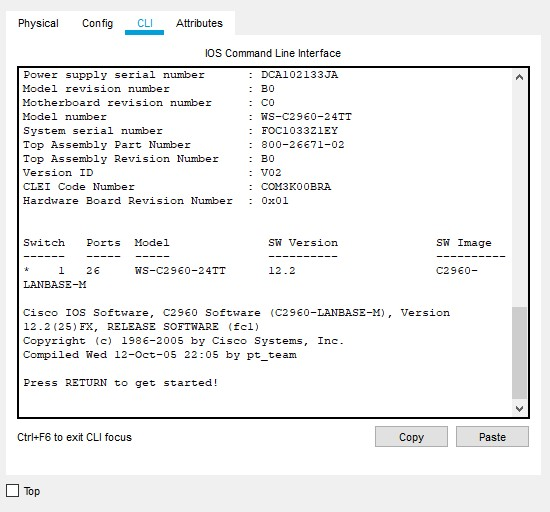
\includegraphics[scale=0.5]{cli.jpg}
	\caption{CLI en Packet Tracer}
\end{figure}

¿Qué es el CLI?, CLI (Command Line Interface) es una interfaz de linea de comandos que permite configurar un dispostivo de red. Allí podremos cambiar las configuraciones y poder tener control del dispositivo.

Para habilitar la entrada de comandos ingresamos la siguiente instrucción:
\begin{lstlisting}[frame=single]
enable	
\end{lstlisting}

Existe tres tipos de usuarios dentro del CLI, los cuales son:
\begin{enumerate}
	\item Usuario Normal ( $>$ )
	\item Usuario Privilegiado ($\#$), es un modo de solo lectura. \\
	Para saber los comandos que se pueden usar en modo privilegiado ingresamos el siguiente comando "\textit{?}"
	\item Modo de configuración global ("nombre\_del\_dispositivo"(config)$\#$)
\end{enumerate}

\newpage

Para ver todas las configuraciones actuales de Switch ingresamos el comando:
\begin{lstlisting}[frame=single]
	show running config
\end{lstlisting}

Para entrar al usuario de modo de configuración global ingresamos:
\begin{lstlisting}[frame=single]
	configure terminal
\end{lstlisting}

\subsection{Configuraciones Básicas}
Cuando se administan redes se requiere de poder realizar una configuración remota al Switch, siempre por el protocolo SSH, por lo tanto en estas configuraciones básicas mostradas a continuación se incluyen también las configuraciones básicas que se requieren tanto para el Switch como para la conexión SSH
Para configurar un Switch debemos ingresar al usuario de configuración global.
\begin{enumerate}
	
	\item[SW] Cambiar el nombre del switch
	\begin{lstlisting}[frame=single]
hostname "nombre"
	\end{lstlisting}
	
	\item[SSH] Configurar un nombre de dominio
	\begin{lstlisting}[frame=single]
ip domain name "nombre_del_dominio"
	\end{lstlisting}
	
	\item[SSH] Generar clave de encriptación para SSH
	\begin{lstlisting}[frame=single]
crypto key generate rsa
	\end{lstlisting}
	
	\item[SSH] Definir la cantidad de bits para la llave, en este caso ingresamos 2048bits que es el tipo más fuerte de encriptación
	\begin{lstlisting}[frame=single]
How many bits in the modulus: 2048
	\end{lstlisting}
	
	
	
\end{enumerate}
	
\end{document}